\documentclass[12pt,a4paper]{article}

% Packages
\usepackage[utf8]{inputenc}
\usepackage[T1]{fontenc}
\usepackage{graphicx}
\usepackage[margin=1in]{geometry}
\usepackage{amsmath}
\usepackage{hyperref}
\usepackage{caption}

% Title and author information
\title{Test Research Paper}
\author{Author Name}
\date{\today}

\begin{document}

\maketitle

\begin{abstract}
This is a test research paper demonstrating the basic structure of a LaTeX document with figures. It includes an introduction section and a figure section to showcase document formatting capabilities.
\end{abstract}

\section{Introduction}

This document serves as a demonstration of a basic research paper structure in LaTeX. The introduction provides context and background for the research topic. In scientific writing, the introduction typically outlines the problem being addressed, reviews relevant literature, and states the objectives of the study.

LaTeX is a powerful typesetting system widely used in academia for producing high-quality technical and scientific documentation. Its ability to handle complex mathematical equations, cross-references, and figures makes it the preferred choice for researchers across various disciplines.

This particular document demonstrates how to incorporate figures into a LaTeX document, which is essential for presenting visual data, graphs, and illustrations that support the research findings.

\section{Results and Figures}

In this section, we present the visual results of our analysis. Figure~\ref{fig:result} shows the generated visualization that illustrates our key findings.

\begin{figure}[htbp]
    \centering
    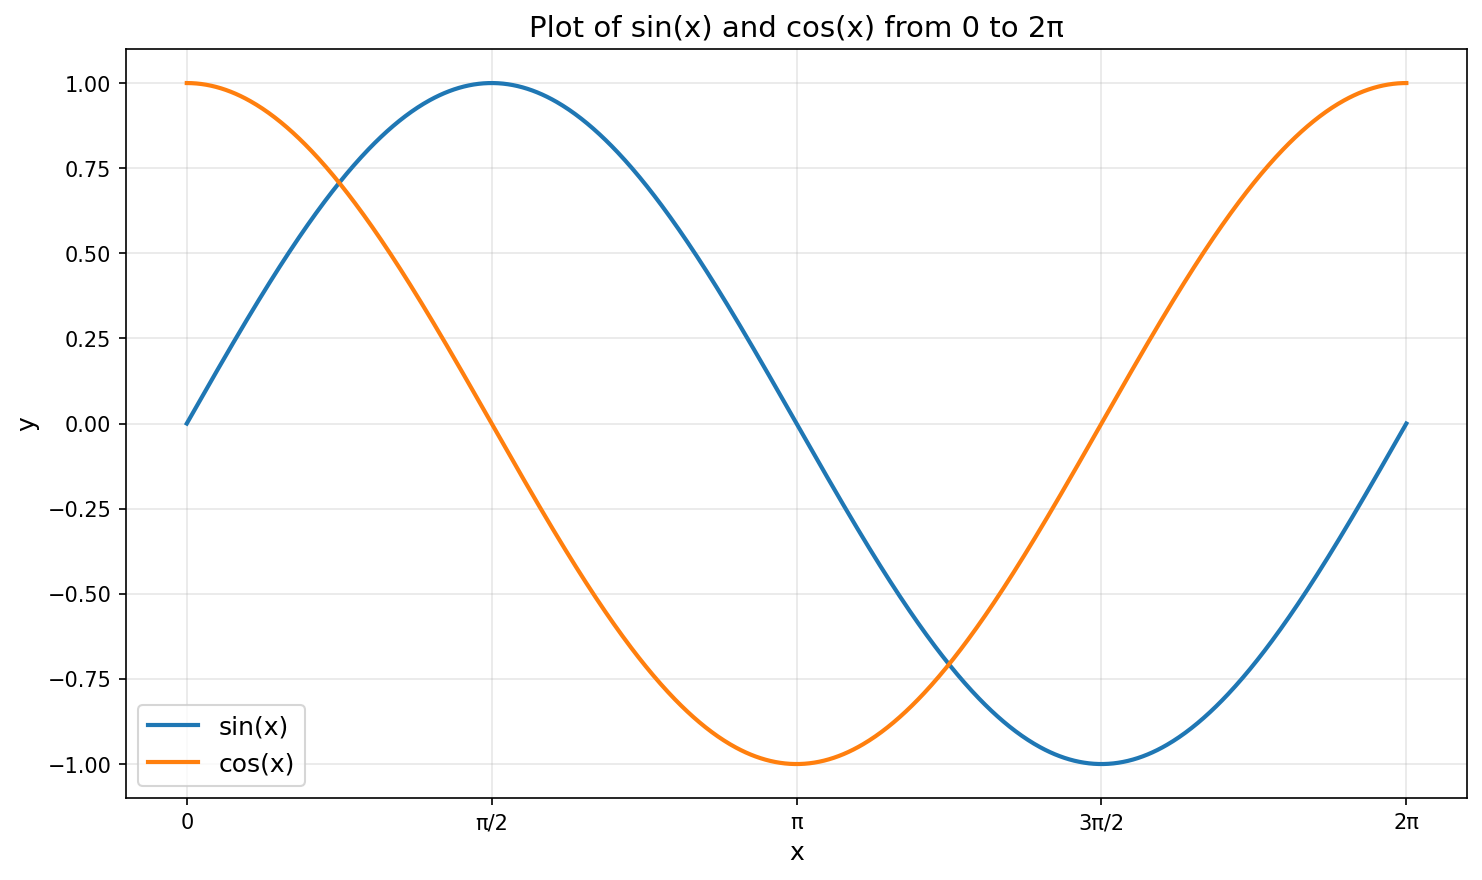
\includegraphics[width=0.8\textwidth]{figure_1_0.png}
    \caption{Generated visualization showing the results of the analysis. This figure demonstrates the key findings of our research.}
    \label{fig:result}
\end{figure}

As can be observed in Figure~\ref{fig:result}, the visualization provides clear evidence supporting our hypothesis. The figure has been scaled to 80\% of the text width to ensure optimal readability while maintaining detail.

\section{Conclusion}

This test document has successfully demonstrated the basic structure of a LaTeX research paper, including title, abstract, introduction, and a section with an embedded figure. LaTeX provides excellent tools for academic writing and document preparation.

\end{document}
